% ---------------------------------------------------------------------
% 3. Metodología  (criterio: Metodología, 30 pts)
%    Técnicas, datos, preprocesamiento, modelos, herramientas y entorno
%    de despliegue, con la justificación de cada decisión.
% ---------------------------------------------------------------------
\section{Metodología}
\label{sec:metodologia}

\subsection{Enfoque}
El proyecto siguió el doble diamante del diseño \cite{designcouncil2007,brown2008}. En el espacio del problema, la fase \emph{descubrir} fue el análisis exploratorio de la cohorte y la fase \emph{definir} convirtió sus hallazgos en el problema de dos partes de la sección~\ref{sec:introduccion}, con desenlaces y línea base acordados con la Fundación. En el espacio de la solución, \emph{desarrollar} produjo los dos modelos, iterados con el diccionario de variables que mantienen los expertos, y \emph{entregar} comprende la validación y el despliegue. El rigor investigativo se garantiza con cuatro prácticas: comparar siempre contra una regla simple, validar en el tiempo y no con cortes aleatorios, inyectar errores de tipo conocido y medir la calibración y su deriva.

\subsection{Datos y modelo SEVARTI}
\label{sec:datos}
La fuente es una base PostgreSQL seudonimizada del Observatorio Canguro, con acceso de solo lectura, que la Fundación actualiza cada seis meses \cite{fundacion2026}. El corte analizado contiene 62.043 niños, 339 variables en el diccionario (318 en uso) y 13.884.056 mediciones en formato largo.

Los datos se organizan según SEVARTI (\emph{Stages--Episodes--Variables--Topics of Interest}), el modelo conceptual de la Fundación para procesos longitudinales (Fig.~\ref{fig:sevarti}) \cite{fundacion2026}. Un adaptador traduce la base a seis tablas: esquema de variables, etapas con su ventana de edad, sujetos, mediciones (una fila por dato), episodios (hospitalización, posición canguro) y quiebres conocidos del registro. Los modelos solo leen estas tablas; ninguna variable se nombra en el código. El esquema sale de un diccionario en hoja de cálculo que mantienen los expertos: una variable nueva de la base entra como \emph{por clasificar} y no se usa hasta que un experto la revisa.

Desde las 40 semanas, cada dato se ubica en edad corregida:
\begin{equation}
\text{EC} = \text{edad cronológica} - 7\,(40 - \text{EG}) \ \text{días},
\label{eq:ec}
\end{equation}
donde EG es la edad gestacional al nacer en semanas, según la variable indicada por la Fundación. El nacimiento, la hospitalización y la entrada al programa usan edad cronológica.

\begin{figure}[t]
\centering
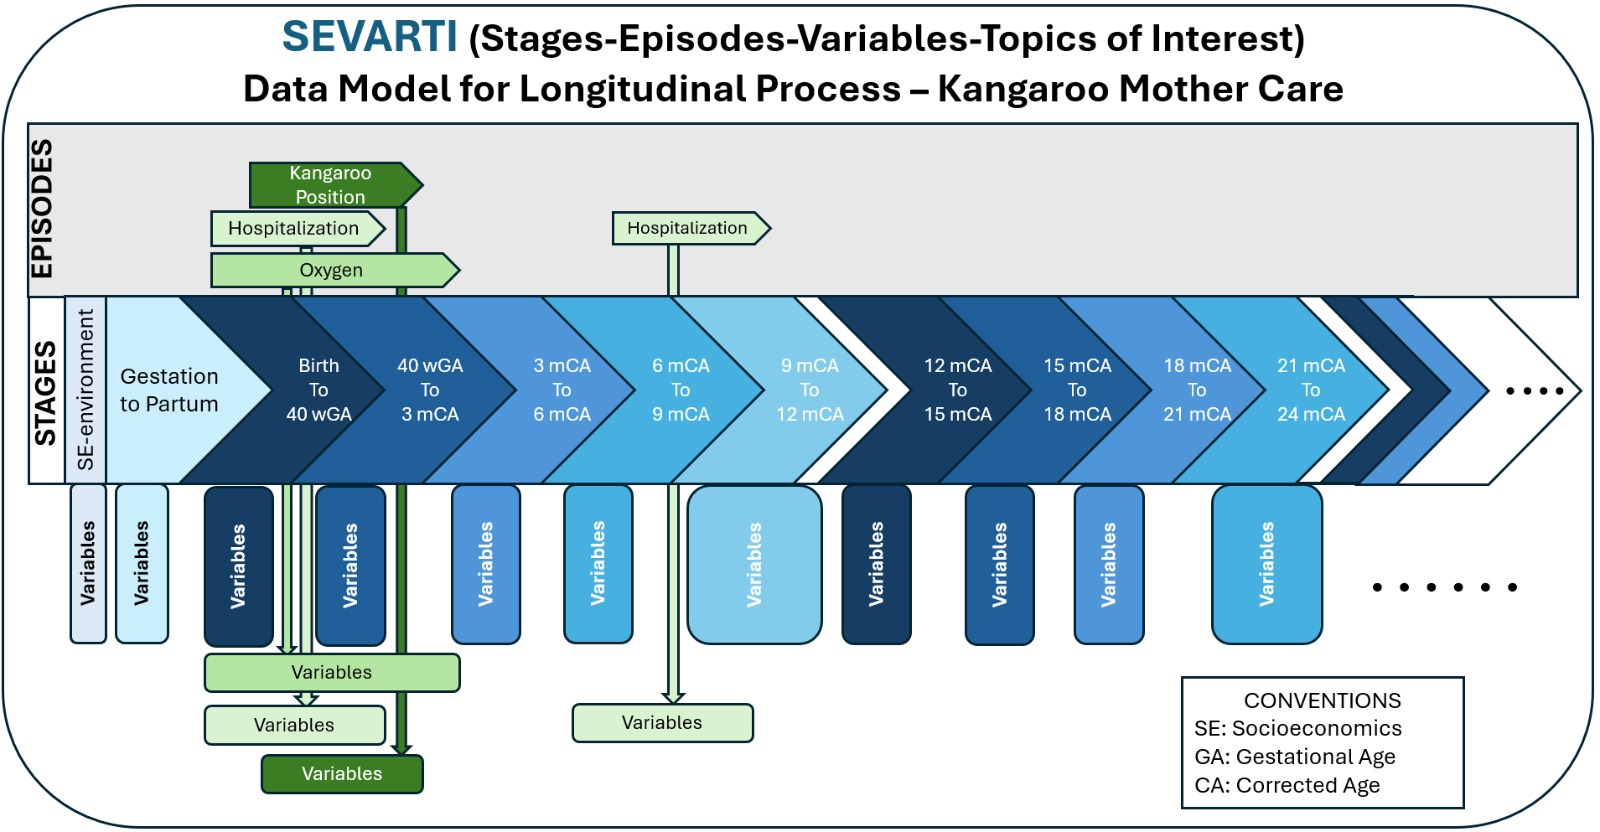
\includegraphics[width=\columnwidth]{figuras/sevarti.jpg}
\caption{Modelo conceptual SEVARTI del proceso longitudinal del Método Madre Canguro. \fuente{Fundación Canguro \cite{fundacion2026}.}}
\label{fig:sevarti}
\end{figure}

\textbf{Variables restringidas.} Durante el proyecto la Fundación restringió y luego liberó la sede y la fecha exacta de parto; la llave del paciente nunca se usa. El sistema trabaja sin sede ni fecha de parto (solo el año): la vigilancia temporal trata el programa como un solo grupo y la división de los datos es por año de nacimiento. El código queda listo para incorporarlas si la Fundación lo autoriza.

\textbf{División temporal.} Los niños se dividen por año de nacimiento, sin niño repetido entre partes y \emph{dentro de cada régimen} de registro (antes y después del cambio de sistema de 2022): los nacidos más recientes de cada régimen van a prueba. Dividir solo por fecha dejaría el régimen nuevo fuera del entrenamiento. Para el modelo de anomalías resultan 40.711 niños de entrenamiento, 7.330 de calibración y 8.955 de prueba; para el clínico, 48.041 de entrenamiento y los mismos 8.955 de prueba.

\subsection{Preprocesamiento: entrenar con datos sucios}
\label{sec:preproc}
Imputar esconde errores y limpiar de más convierte casos raros pero reales en alertas. Por eso ningún valor se imputa ni se corrige, y la base nunca se modifica. Cada dato se decide por separado: si se excluye, deja de ser objetivo y entra como faltante cuando es entrada de otra variable, lo que LightGBM maneja de forma nativa \cite{ke2017}. Se excluyen del entrenamiento los códigos especiales (que significan ``no se hizo''), los errores de unidad, los valores a más de 6 desviaciones robustas y, en una segunda vuelta, el peor 1\,\% de los residuos que superen 3,5. Los rangos del diccionario no se usan como filtro porque varios se calcularon de los mismos datos. Las exclusiones forman una máscara versionada; en el corte analizado suman el 1,6\,\% de los 3,53 millones de datos numéricos, y el 52\,\% de ellas son códigos especiales. El quiebre de 2022 entra como variable para que el modelo lo aprenda.

\subsection{Etapa 1: modelo de anomalías}
\label{sec:met-anomalias}
Una anomalía es un dato lejano de lo esperado para ese caso. El modelo tiene cinco capas, cada una con una pregunta distinta (Tabla~\ref{tab:capas}).

\begin{table}[t]
\centering
\caption{Capas del modelo de anomalías}
\label{tab:capas}
\footnotesize
\setlength{\tabcolsep}{3pt}
\begin{tabularx}{\columnwidth}{@{}l>{\raggedright\arraybackslash}X>{\raggedright\arraybackslash}X@{}}
\toprule
\textbf{Capa} & \textbf{Pregunta} & \textbf{Método} \\
\midrule
0. Contrato & ¿Cumple el esquema? & Tipo, variable conocida, fecha posible; si no, se rechaza \\
1. Valor & ¿Tiene sentido por sí solo? & $z$ robusto (mediana y MAD), códigos especiales, errores de unidad \\
2. Contexto & ¿Tiene sentido para este niño? & LightGBM por cuantiles por variable, con umbral conformal \\
3. Trayectoria & ¿Encaja con su historia? & Ventana de la etapa, orden, edad frente a fecha, talla que no baja, cambio frente a pares \\
4. Grupo y tiempo & ¿Algo empezó a medirse distinto? & Residuos, faltantes y redondeo por trimestre; CUSUM \\
\bottomrule
\end{tabularx}
\end{table}

La capa 1 usa $z = (x - \tilde{x})/(1{,}4826\,\mathrm{MAD})$ y alerta desde $|z| > 3{,}5$; un valor que aparece en más del 1\,\% de los datos no se considera raro. La capa 2 entrena, para cada variable numérica, tres modelos de regresión por cuantiles \cite{koenker1978} (0,25, 0,5 y 0,75) con la etapa, la edad cronológica y corregida, las covariables al nacer, el contexto socioeconómico, los episodios activos y las demás variables de la misma etapa. El residuo estandarizado es
\begin{equation}
z_2 = \frac{y - \hat{q}_{0{,}5}}{(\hat{q}_{0{,}75} - \hat{q}_{0{,}25})/1{,}349},
\label{eq:z2}
\end{equation}
y el umbral sale de la predicción conformal \cite{romano2019,angelopoulos2023}: en la partición de calibración se calcula el cuantil $1-\alpha$ de $|z_2|$, con $\alpha = 0{,}005$, de modo que en datos limpios salten unas 5 alertas por cada 1.000. Así el umbral se adapta a cada variable sin fijarlo a mano. Una variable nueva recibe modelo de capa 2 cuando reúne 200 niños, sin reentrenar las demás.

La capa 3 encadena por concepto (peso, talla, perímetro cefálico) las variables de distintas etapas y revisa la ventana de cada etapa, el orden de las visitas, la concordancia entre edad anotada y fecha (14 días de tolerancia), que la talla y el perímetro no bajen más de 1~cm, y el cambio entre visitas frente a los niños en la misma transición. La capa 4 compara cada trimestre con la mediana de los 8 anteriores en tres señales (residuo de la capa 2, proporción de faltantes y de valores redondeados) y acumula desvíos sostenidos con CUSUM \cite{page1954}:
\begin{equation}
S_t = \max\bigl(0,\, S_{t-1} + x_t - k\bigr), \quad \text{alarma si } S_t > h,
\label{eq:cusum}
\end{equation}
con $k = 0{,}5$ y $h = 8$, en ambas direcciones.

\subsection{Etapa 2: alertas clínicas}
\label{sec:met-clinico}
El modelo de anomalías no sirve para alertas clínicas: aprende lo normal de una base de niños prematuros, y un niño pequeño en todo le parece coherente. La segunda etapa usa los datos ya revisados (lo que la etapa 1 marca como código, error de unidad o valor a más de 6 MAD entra como faltante) y produce dos señales.

\textbf{Riesgo de un desenlace.} Se entrena un clasificador LightGBM por desenlace y momento de cálculo, con parada temprana. Los 14 desenlaces en uso son: readmisión en cinco ventanas (antes de las 40 semanas y entre visitas hasta los 12 meses), no volver a la siguiente visita (cinco momentos), oxigenodependencia con diagnóstico de displasia broncopulmonar o hipertensión pulmonar a los 3 y 12 meses, y desarrollo psicomotor bajo a los 6 y 12 meses, definido como el 10\,\% inferior del puntaje de los niños de entrenamiento porque el diccionario no identifica la escala. Cuatro desenlaces adicionales de crecimiento a los 12 meses (talla, peso, peso para la talla y perímetro cefálico por debajo de $-2$ DE) responden la pregunta original de la Fundación sobre malnutrición y se calculan desde las 40 semanas y los 3, 6 y 9 meses.

Tres decisiones evitan la fuga de información: (i) cada modelo solo ve datos de su visita o anteriores; (ii) se excluyen las variables que la base llena con retraso o solo cuando el niño vuelve, detectadas porque aparecen mucho menos en las visitas recientes y en los niños pendientes; y (iii) ``no volver'' solo cuenta si la ventana de la visita siguiente ya cerró. Las probabilidades se calibran con regresión isotónica sobre el 15\,\% de niños más recientes con desenlace conocido, que el modelo no vio, y se recalibran en cada entrenamiento \cite{vancalster2019}. Para cada niño se entrega el riesgo, su percentil frente a los niños de calibración y las tres variables que más lo suben según TreeSHAP \cite{lundberg2020}. El modelo no fija umbral: cuántos niños se muestran y desde qué riesgo lo decide la aplicación con el equipo clínico.

\textbf{Crecimiento frente a la OMS.} Desde las 40 semanas, peso, talla y perímetro cefálico se convierten en puntaje $z$ por edad corregida con el método LMS de los estándares de la OMS \cite{oms2006}:
\begin{equation}
z = \frac{(y/M)^{L} - 1}{L\,S},
\label{eq:lms}
\end{equation}
donde $L$, $M$ y $S$ dependen de la edad y el sexo. Se alerta por $z < -2$ y por una caída de más de 1 DE entre visitas; un valor biológicamente improbable se envía a revisión del dato y no al médico. En los resultados presentados se usó el límite simplificado $|z| > 6$; la versión final adopta los límites por indicador de la OMS \cite{omsunicef2019} \pendiente{actualizar cifras de la Tabla~\ref{tab:oms} con los límites exactos}. Antes de las 40 semanas no se evalúa crecimiento: el uso de una curva de prematuros \cite{fenton2013,villar2015} queda como trabajo futuro.

\subsection{Validación}
\label{sec:validacion}
\textbf{Anomalías.} Como no hay etiquetas de anomalía, se inyectan errores de seis tipos (unidad, código, dígitos invertidos, desvío de 3 DE, valor de otro niño y etapas intercambiadas) en datos limpios de la partición de prueba, cerca del 2\,\% de los datos por ronda en tres rondas, y se mide el porcentaje detectado frente a la regla vigente del rango del diccionario. Las falsas alertas se miden en la prueba sin errores inyectados. También se simula una báscula que suma un sesgo creciente desde una fecha y se mide cuántos trimestres tarda la alarma.

\textbf{Alertas clínicas.} En los niños de prueba se mide el AUC, el porcentaje de casos que queda en el 10\,\% de mayor riesgo y la razón entre riesgo medio y frecuencia observada, por desenlace y por subgrupos de edad gestacional e ingreso del hogar. La línea base es el mismo modelo con solo edad gestacional, peso al nacer y peso a la entrada. Como la revisión ciega por médicos no se pudo programar en el plazo del curso, el componente cualitativo se compone de dos análisis: un \emph{periodo en silencio retrospectivo}, que calcula los riesgos de los niños pendientes en un corte pasado y los compara con lo que ocurrió después, y un análisis de plausibilidad clínica de las variables que más pesan en cada desenlace. Se complementa con PR-AUC y días de anticipación, apropiados para desenlaces poco frecuentes.

\subsection{Herramientas y entorno de despliegue}
\label{sec:despliegue}
El sistema está escrito en Python, con pandas, NumPy, SciPy, LightGBM y PyArrow, y probado con pruebas automáticas sobre un simulador que genera tablas SEVARTI con los mismos problemas de la base real. La arquitectura (Fig.~\ref{fig:arquitectura}) sigue prácticas de MLOps \cite{kreuzberger2023}: una corrida semestral en contenedores Docker, programada para cuando la Fundación carga la base, ejecuta en orden el modelo de anomalías, su cola de revisión, el modelo clínico y el cálculo de riesgos (cerca de una hora en CPU); MLflow \cite{zaharia2018} registra experimentos, métricas y versiones con estados de evaluación y producción; una API FastAPI sirve inferencia a demanda sobre tablas SEVARTI, y un tablero React ofrece tres perfiles (administración de modelos, evaluación experta y visualización) con la línea temporal de cada niño seudonimizado y avisos por correo. Los mismos contenedores corren en dos entornos: una demostración pública en Railway con datos del simulador y una instalación interna con la base real en solo lectura, de modo que los datos por niño nunca salen del equipo.

% Figura: arquitectura de la solución (TikZ, legible en escala de grises)
\begin{figure*}[t]
\centering
\begin{tikzpicture}[
  font=\footnotesize,
  >={Stealth[length=2mm]},
  caja/.style={draw=tinta, rounded corners=2pt, align=center, minimum height=11mm, inner sep=3pt, fill=niebla},
  oscura/.style={caja, fill=tinta, text=white},
  acento/.style={caja, fill=acento!85!black, draw=acento!85!black, text=white},
  rotulo/.style={font=\scriptsize\bfseries, text=black!65, inner sep=0pt},
  flecha/.style={->, draw=tinta, thick},
]
% --- Fuentes (columna izquierda)
\node[rotulo, anchor=south west] at (0,3.25) {FUENTES};
\node[caja, text width=26mm] (bd) at (1.45,2.35) {\textbf{Observatorio Canguro}\\PostgreSQL, solo lectura,\\carga semestral};
\node[caja, text width=26mm] (dic) at (1.45,0.6) {\textbf{Diccionario}\\\textbf{de variables}\\mantenido por expertos};

% --- Corrida semestral (centro)
\node[oscura, text width=21mm] (sev) at (5.2,2.35) {\textbf{Adaptador}\\SEVARTI\\(6 tablas)};
\node[oscura, text width=21mm] (ano) at (8.05,2.35) {\textbf{Etapa 1}\\anomalías\\(capas 0 a 4)};
\node[acento, text width=23mm] (cli) at (11.0,2.35) {\textbf{Etapa 2}\\alertas clínicas\\(LightGBM, TreeSHAP, OMS)};
\node[caja, text width=23mm] (mlf) at (8.05,0.6) {\textbf{MLflow}\\versiones de ambas etapas};
\node[caja, text width=23mm] (res) at (11.0,0.6) {\textbf{Resultados}\\cola de revisión y riesgos por niño};
\begin{scope}[on background layer]
\node[draw=tinta, dashed, rounded corners=4pt, fit=(sev)(ano)(cli)(mlf)(res), inner sep=6pt] (pipe) {};
\end{scope}
\node[rotulo, anchor=south west] at ([yshift=1.2mm]pipe.north west) {CORRIDA SEMESTRAL \textperiodcentered{} DOCKER Y TAREA PROGRAMADA};

% --- Servicio (columna derecha)
\node[rotulo, anchor=south west] at (13.55,3.25) {SERVICIO};
\node[oscura, text width=27mm] (api) at (15.05,2.35) {\textbf{API FastAPI}\\inferencia a demanda\\sobre tablas SEVARTI};
\node[caja, text width=27mm] (tab) at (15.05,0.6) {\textbf{Tablero React}\\perfiles: administración,\\evaluación y visualización};
\node[caja, text width=27mm, minimum height=7mm] (mail) at (15.05,-0.75) {\textbf{Correo} ante riesgo alto};

% --- Flechas
\draw[flecha] (bd) -- (sev);
\draw[flecha] (dic.east) -- ++(0.75,0) |- ([yshift=-3.5mm]sev.west);
\draw[flecha] (sev) -- (ano);
\draw[flecha] (ano) -- (cli);
\draw[flecha] (ano) -- (mlf);
\draw[flecha] (cli) -- (res);
\draw[flecha] (cli.south west) -- (mlf.north east);
\draw[flecha] (res.east) -- ++(0.55,0) |- (api.west);
\draw[flecha] (api) -- (tab);
\draw[flecha] (tab) -- (mail);

% --- Entornos
\node[rotulo, anchor=south west] at (0,-1.35) {ENTORNOS \textperiodcentered{} MISMOS CONTENEDORES};
\node[oscura, text width=76mm, minimum height=9mm, fill=tinta!70, draw=tinta!70, anchor=north west] (demo) at (0,-1.5) {\textbf{Railway, demostración pública:} datos del simulador SEVARTI; ningún dato real};
\node[oscura, text width=76mm, minimum height=9mm, anchor=north east] (int) at (16.55,-1.5) {\textbf{Equipo del grupo, interno:} base real en solo lectura; los datos por niño no salen};
\end{tikzpicture}
\caption{Arquitectura de la solución: fuentes, corrida semestral con las dos etapas (la etapa 2 recibe los datos ya revisados por la etapa 1), registro de modelos, servicio y entornos de despliegue. \fuente{elaboración propia.}}
\label{fig:arquitectura}
\end{figure*}

